\section{Interaural Time Difference\\ \& Interaural Intensity Difference}
\label{sec:ITD}

Følgende beskrivelse er baseret på en lydkilde som ligger væk fra kroppens sagitale plan, dvs. i en azimuth $ \ne 0^\circ$. 

\subsection{ITD}
Interaural Time Difference (ITD) er beregningen af tidsforskellen fra lyden rammer det første øre til det andet øre. Dette er især hørbart ved frekvenser under 1.5kHz hvor bølgelængden $\lambda$ er større end afstanden mellem ørerne som er omkring 23cm, som vist i nedenstående beregning, hvor c er lydens hastighed i luft ved $20^\circ C $.

\( f=1500Hz \hspace{1cm}  c=343\frac{m}{s} \hspace{1cm} t = \frac{1}{f} = 0.6ms  \\ \lambda = t \cdot c = 0.23m \)

Ved disse frekvenser vil afstanden mellem ørerne medvirke en faseforskel, som bruges til at lokalisere azimuth. Ved højere frekvenser, vil faseforskellen være svær at begrænse (hvis overhovedet eksisterende), men ved mellemtone og høje frekvenser opstår der diffration rundt om hovedet, hvorved der kastes en akustisk skygge som vist på figur \ref{fig:ITD}

\figur{.8}{ITD}{Venstre side viser ITD delay mellem højre og venstre øre ved lave frekvenser. Højre side viser den akustiske skygge ved mellem- og høje-frekvenser\cite{ITDPic}}{ITD}

For at skabe en digital ITD, sættes et delay mellem hhv højre og venstre signal som svarer til den ønskede azimuth ud fra en fastsat afstand mellem ørerne på 23cm.

\subsection{IID}

Interaural Intensity Difference (IID), eller Interaural Level Difference (ILD) er forskellen i lydsignalets amplitude ved hhv højre og venstre øre hhv før og efter påvirkning fra den akustiske skygge. Pga den akustiske skygge, vil lydsignalets amplitude blive dæmpet, og ud fra denne amplitude forskel mellem højre og venstre øre, kan hjernen afgøre lydkildens azimuth og elevation.

Overlappet mellem om hjernen reagerer mest på ITD og IID ligger - som vist på figur \ref{fig:itdiid} - omkring 1kHz-2kHz  afhængig af den eksakte azimuth og elevation.

I dette projekt er IID integreret i hrtf'erne som beskrives i afsnit \ref{sec:HRTF}.

\begin{figure}
	\centering
	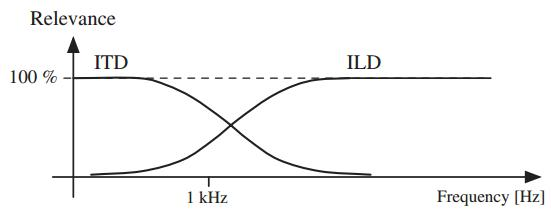
\includegraphics[width=0.7\linewidth]{All_Pics/ITDIID}
	\caption{Overlap mellem vigtigheden af ITD og IID for opfattelsen af et lydobjekts placering \cite{SpatialBook}}
	\label{fig:itdiid}
\end{figure}
